\documentclass[a4paper]{article}
\usepackage{amsmath}
\usepackage{amsfonts}
\usepackage[english]{babel}
\usepackage{fancyhdr}
\let\oldAuthor\author
\renewcommand{\author}[1]{\newcommand{\myAuthor}{#1}\oldAuthor{#1}} 
\usepackage{listings}
\usepackage{enumitem}
\usepackage{xcolor}
\usepackage[nolist]{acronym}
\setlist[description]{leftmargin=0.4cm}
\usepackage{graphicx}
\usepackage{hyperref}

\begin{document}

\definecolor{mGreen}{rgb}{0,0.6,0}
\definecolor{mGray}{rgb}{0.5,0.5,0.5}
\definecolor{mPurple}{rgb}{0.58,0,0.82}
\definecolor{backgroundColour}{rgb}{0.95,0.95,0.92}

\lstdefinestyle{CStyle}{
    backgroundcolor=\color{backgroundColour},   
    commentstyle=\color{mGreen},
    keywordstyle=\color{magenta},
    numberstyle=\tiny\color{mGray},
    stringstyle=\color{mPurple},
    basicstyle=\ttfamily,
    breakatwhitespace=false,         
    breaklines=true,                 
    captionpos=b,                    
    keepspaces=true,                 
    numbers=left,                    
    numbersep=5pt,                  
    showspaces=false,                
    showstringspaces=false,
    showtabs=false,                  
    tabsize=2,
    language=C
}
\lstset{style=CStyle}

%---------------------------------------------------------
%Fill in:
%1. Title of lab. 
%2. Student names and corresponding Email addresses. If many separate 
%---------------------------------------------------------
\title{Operating Systems - Assignment 2}
\author{Ansgar Lemke (ens21ale)}
\date{} %<-- LEAVE EMPTY! 
\begin{titlepage}
\maketitle 
%---------------------------------------------------------
%Fill in:
%1. Course name
%2. Supervisor name(s), if many separate them by comma.
%---------------------------------------------------------
\thispagestyle{fancy}
\headheight 35pt 
\lhead{\small Department of Computing Science \\ Ume\aa\ University}
\rhead{\small\today}
\cfoot{Operating Systems \\ Supervisor: Monowar Bhuyan (monowar@cs.umu.se),\\ Sourasekhar Banerjee (sourasb@cs.umu.se)}
\begin{abstract}
%	What was the aim of the experiment? 
A simple scatter-gather functionality will be implemented.
%	What was measured?
The execution speed of the implementation will be compared using different parameters for the scatter-gather function calls to compute the same problem.
%	Which techniques/methods were used? 
This approach uses shared memory and processes to implement the functionality.
%	What are the main results?
Depending on the size of memory, used devices and the computational load of the tasks, there is an optimal number of processes to use.

The source code of this project as well as this report can be found at \href{https://github.com/einansgar/scatter-gather}{https://github.com/einansgar/scatter-gather}.

\end{abstract}

\end{titlepage}
\pagestyle{fancy}
\headheight 35pt 
\rhead{\small\today}
\lhead{\myAuthor}
\cfoot{\thepage}

\section{Description}

scatter-gather is an algorithm to split up a memory area so that multiple processes can work on the same computational problem and combine the results to one field of memory afterwards. MPI implements this functionality as MPI\_Scatter\_Gather, however, this solution aims to be as easy to use as possible. It's only dependencies are standard libraries.

\subsection{Solution}

The library is implemented in C99 which makes it available to many applications. With the used of shared memory but separated areas within for the different processes, questions of synchronization fall apart in most of the implementation. In the scattered phase, the processes work independent of each other and do not need any synchronization or communication which offers a good concurrent environment. 

\subsection{Design Decisions}

Each process is assigned to a segment which corresponds to a certain area of the shared memory. The highest segment is assigned to the parent process. This information can be used to exit all other processes in the end to continue on the parent only. 

One goal is to provide an interface to the user which grants full functionality while being relatively safe by hiding parts that are not relevant for end users. To transmit data from scatter to gather, a static struct is used internally. There are two functions available to be used by the user:

\begin{itemize}
    \item {scatter takes initialization data and parameters and provides a pointer to a location in shared memory for each process to work on. }
    \item {gather ends processes as soon as all of their children have died, except for the root process which has called scatter once. This one is provided with a copy of the shared memory after all the other processes have finished.}
\end{itemize}

Between scatter and gather, multiple processes exist to compute tasks in parallel.

\subsection{Assumptions}

The spawned processes must only work on their own memory section, proc\_memory. They must not change the location of the pointer because then their changes will not be written back. They must strictly remain inside their memory area, otherwise they would write either on memory of another process or even to an invalid location outside the shared memory area.  

It is assumed that all processes take nearly the same amount of time, otherwise, the waiting might take up to the time the slowest process needs to finish plus the time to exit the others. In addition, is assumed that processes do enough work to justify the overhead by process creation and destruction.

\subsection{Limitations}

The amount of available data types is restricted to the basic C types which do not contain any pointers to other memory locations and have a fixed size, e. g. int, char. Inclusion of pointers or other more complex data structures would introduce the problem that these need to be copied to the shared memory as well while it is not known how exactly their structure looks like.

The scatter-gather calls cannot be nested, if scatter is called, gather must follow exactly one time. This greatly simplifies the structure because a lot of the functionality can be hidden from the user. 

On multi-processor systems, the behavior of cache pages might reduce performance when data needs to be copied back again or adjacent memory areas might be synchronized as well out of the interpretation that most users might want to access these as well. The effects of false sharing might also decrease the execution speed. And of course, there is a maximum size of memory that can be used in RAM.

\section{Examples}

To demonstrate the functionality of scatter-gather, two computational problems will be executed with different amounts of processes. The programs will be executed on a Intel\copyright Core\textsuperscript{TM} i7-7500U CPU @ 2.70GHz $\times$ 4. The results on a GPU are expected to be quite different.

\subsection{Arithmetic Operations}
On each segment of memory, a combination of set, scale, add, scale is executed ten times on an array of size 504000. Each number of processes is tested 100 times.

\begin{figure}[ht]
    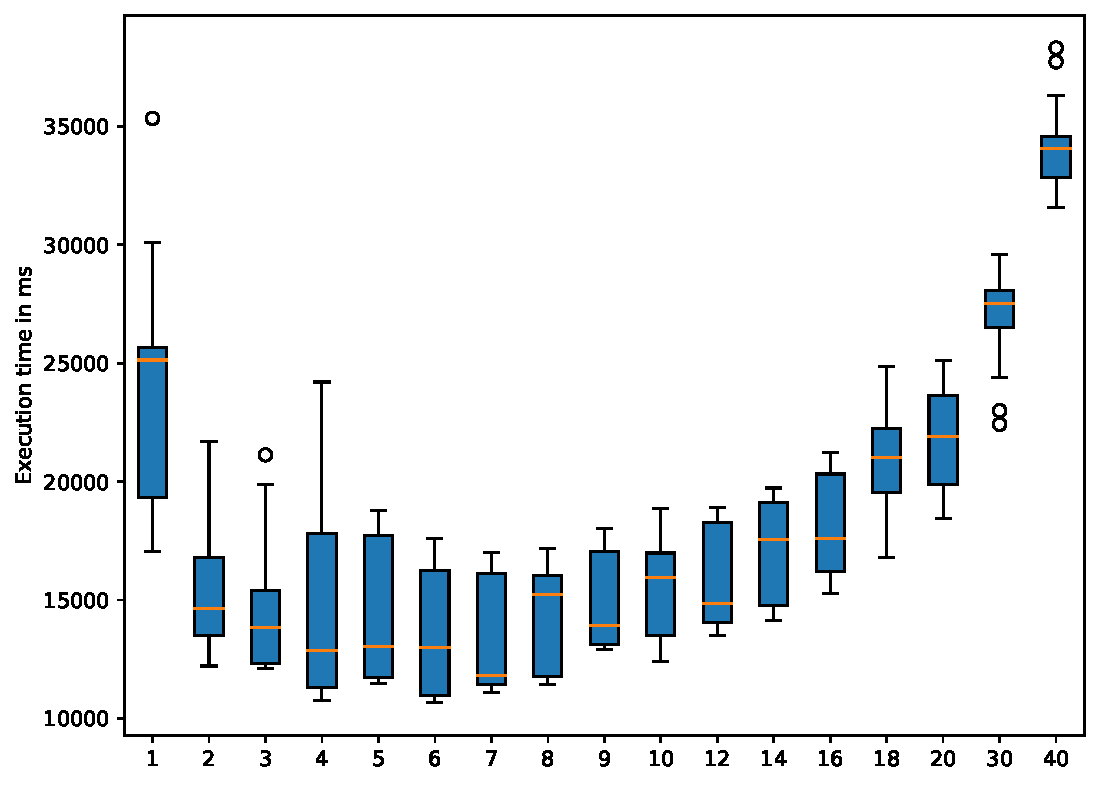
\includegraphics[width=0.8\textwidth]{figs/dump1.pdf}
    \caption{Execution times on arithmetic operations}
    \label{fig:dump1}
\end{figure}

\subsection{Generating Random Numbers}
The segment of process memory is being filled with random numbers. The operation is executed on an array of size 504000. Each number of processes is tested 100 times.

\begin{figure}[ht]
    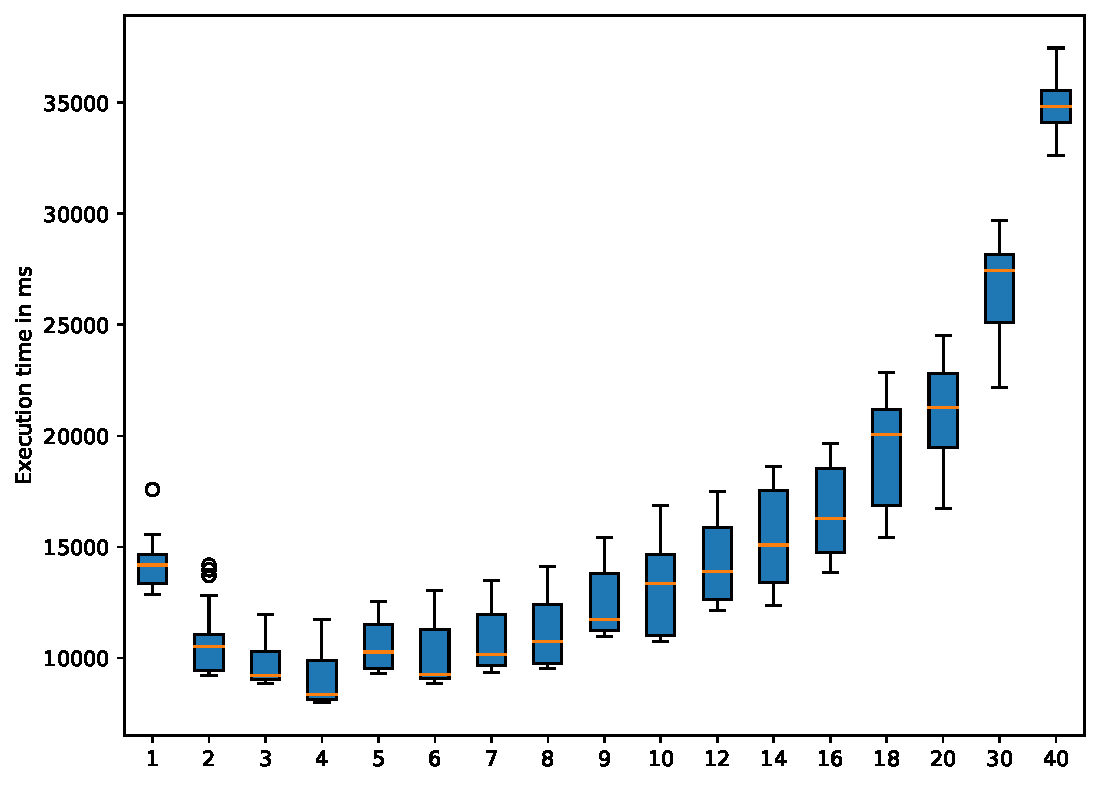
\includegraphics[width=0.8\textwidth]{figs/dump2.pdf}
    \caption{Execution times on generating random numbers}
    \label{fig:dump2}
\end{figure}

\section{Conclusions}

In the chosen setup, creation of more than 10-20 processes results in even worse performance than a single process, marking out the importance of overhead, especially in the fork calls. Depending on the tasks, execution times can be reduced significantly.

% \bibliographystyle{plain}

% \begin{thebibliography}{99}
% 	\bibitem{sched_plot_thickens} Corbet, Jonathan, Schedulers: The Plot Thickens, LWN.net, (April 2007, \href{https://lwn.net/Articles/230574/}{https://lwn.net/Articles/230574/}).
% 	\bibitem{mp_sched} sched(7) Linux User's Manual, Edition 5.3, (February 2022).
%     \bibitem{async} oxnz: Linux Asynchronous I/O (October 13 2016, https://oxnz.github.io/2016/10/13/linux-aio/).
%     \bibitem{nocache} open(2) Linux User's Manual, Edition 5.13, (February 2022).
%     \bibitem{iosched} colin-king et al: IOSchedulers ubuntu wiki (September 2019, https://wiki.ubuntu.com/Kernel/Reference/IOSchedulers).
% \end{thebibliography}

\end{document}
